\chapter{Reglementen \& Voorrangsregels}
\vspace{-120px}
\section*{Wie heeft er voorrang? Denk ook goed na waarom en vul de letter in!}
\begin{table}[h!]
\centering
\begin{tabular}{l|l|l|l|l|l|l|l|l|l|l|l}
\textbf{1} & \textbf{2} & \textbf{3} & \textbf{4} & \textbf{5} & \textbf{6} & \textbf{7} & \textbf{8} & \textbf{9} & \textbf{10} & \textbf{11} & \textbf{12} \\ \hline
 \hspace{0.5 cm} & \hspace{0.5 cm}  & \hspace{0.5 cm} & \hspace{0.5 cm} & \hspace{0.5 cm} & \hspace{0.5 cm} & \hspace{0.5 cm} & \hspace{0.5 cm} & \hspace{0.5 cm} & \hspace{0.5 cm} & \hspace{0.5 cm} & \hspace{0.5 cm}
\end{tabular}
\end{table}
\begin{figure}[h!]
    \centering
    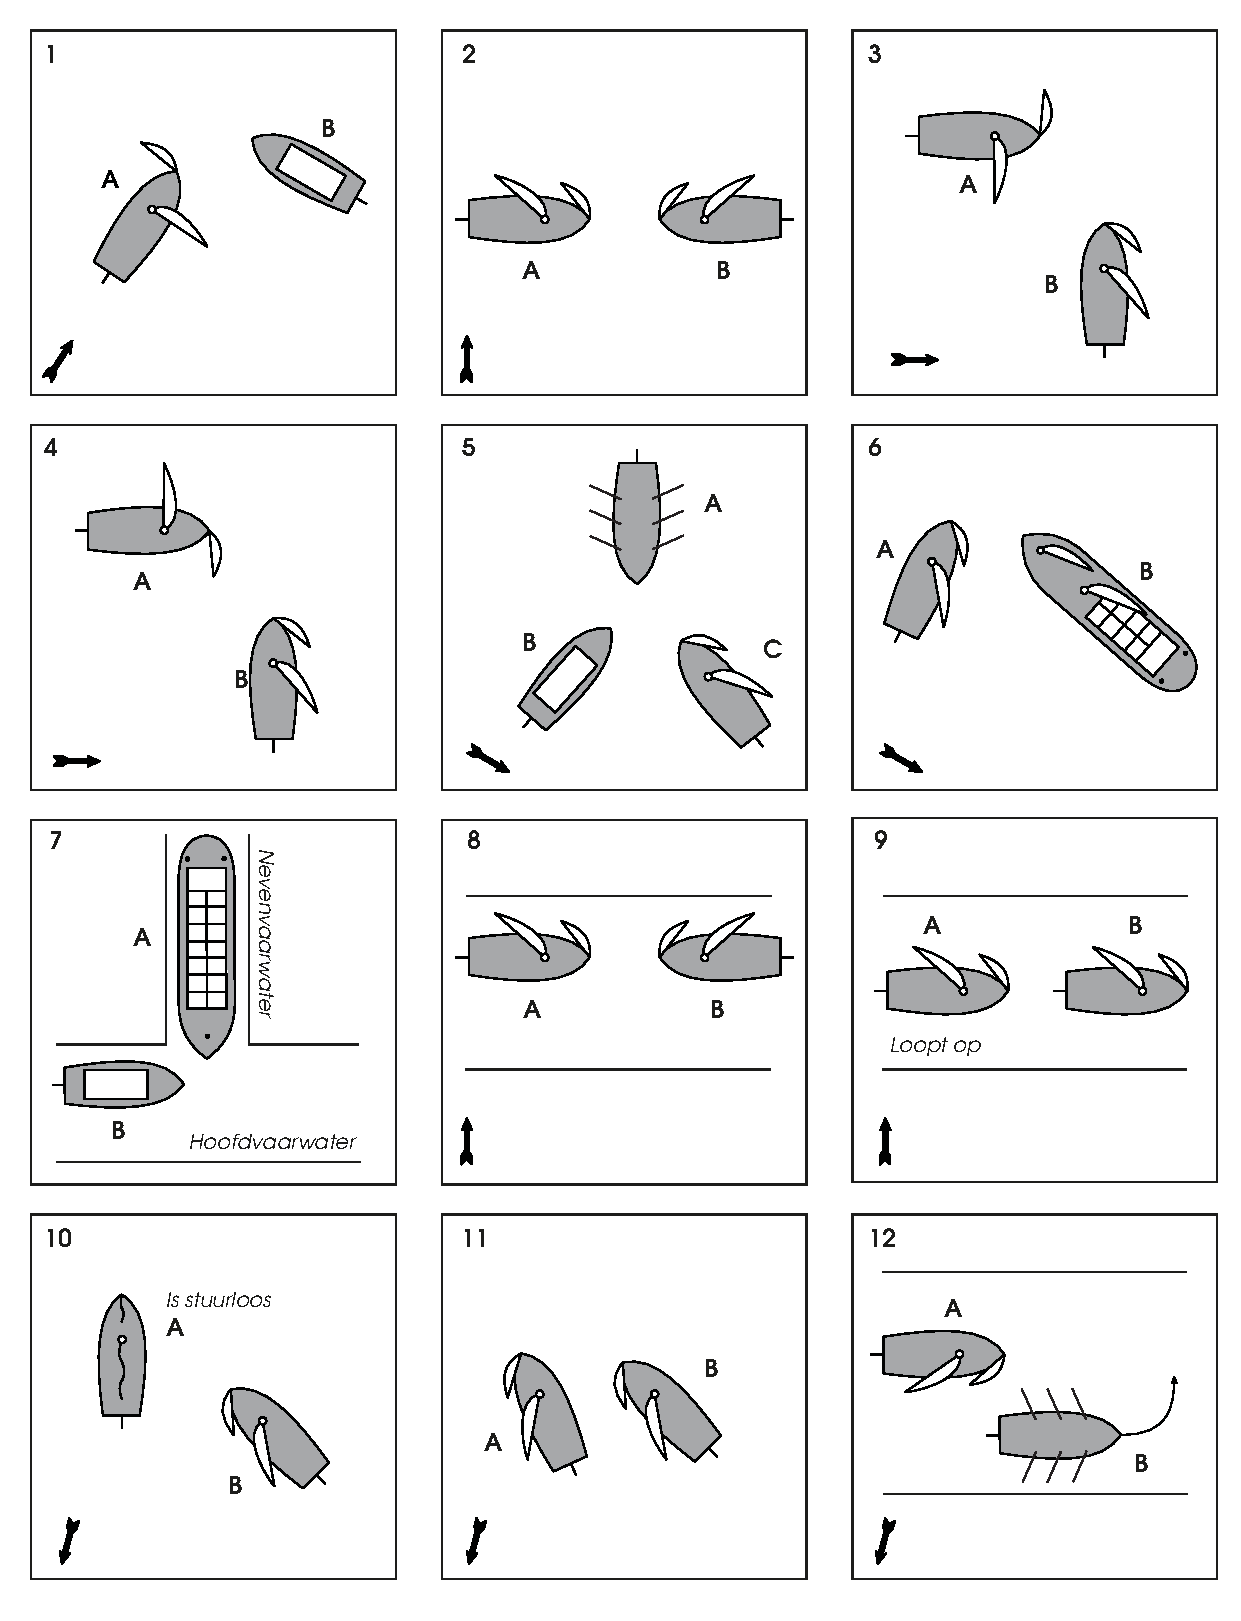
\includegraphics[width=\textwidth]{Hoofdstukken/Oefenvragen/pdf/regelementen_1.pdf}
\end{figure}

\newpage
\begin{table}[h!]
	\centering
	\begin{tabular}{l|l|l|l|l|l|l|l|l|l|l}
		\textbf{13} & \textbf{14} & \textbf{15} & \textbf{16} & \textbf{17} & \textbf{18} & \textbf{19} & \textbf{20} & \textbf{21} & \textbf{22} & \textbf{23} \\ \hline
		\hspace{0.5 cm} & \hspace{0.5 cm}  & \hspace{0.5 cm} & \hspace{0.5 cm} & \hspace{0.5 cm} & \hspace{0.5 cm} & \hspace{0.5 cm} & \hspace{0.5 cm} & \hspace{0.5 cm} & \hspace{0.5 cm} & \hspace{0.5 cm}
	\end{tabular}
\end{table}
\begin{figure}[h!]
    \centering
    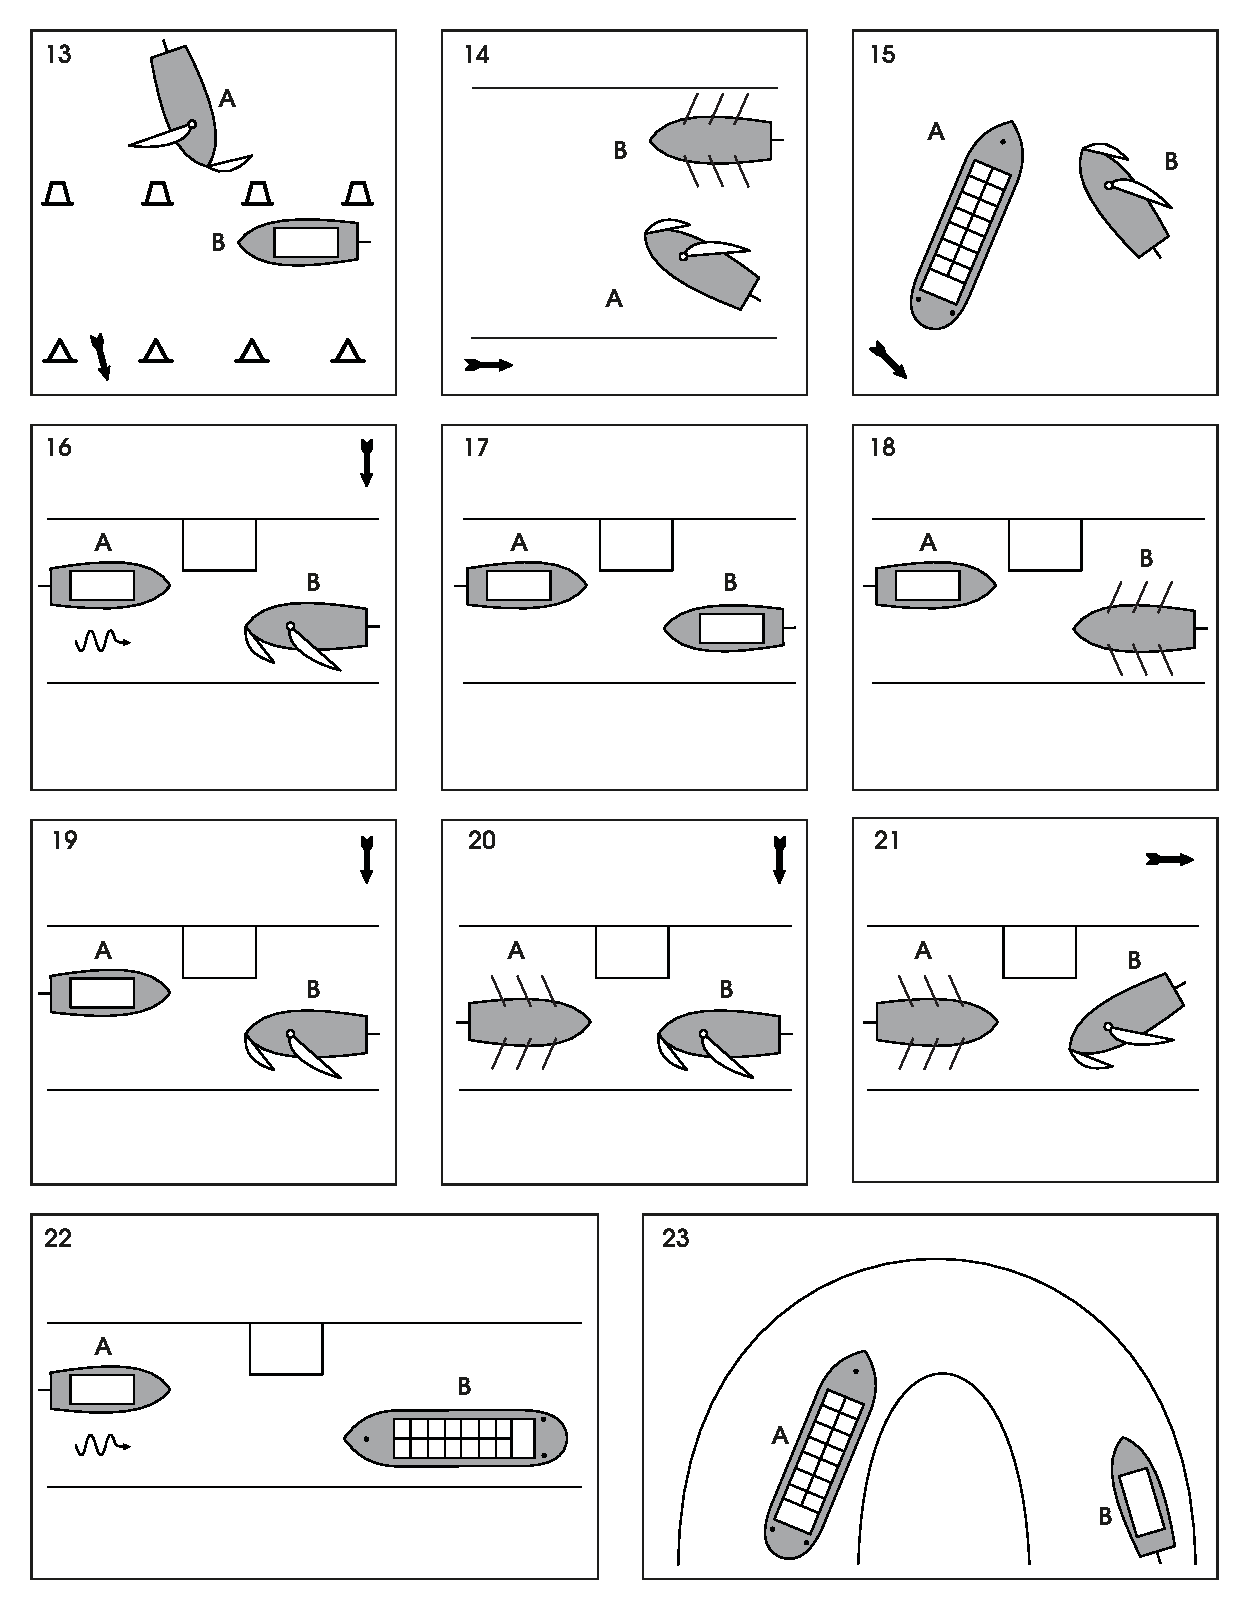
\includegraphics[width=\textwidth]{Hoofdstukken/Oefenvragen/pdf/regelementen_2.pdf}
\end{figure}
\newpage

\question{24}{Wat is de betekenis van het bord in het figuur rechts?}
\vspace*{-0.5cm}
\answerTextPicture{In-, uit-, of doorvaren verboden}{Einde van een verbod of gebod}{Verboden geluidsseinen te maken}{Verplichting voor het bord stil te houden}{Hoofdstukken/Reglementen/pdf/B5.pdf}

\question{25}{Wat betekent het volgende geluidssein: \slong \sspace  \sshort \sspace  \slong }
\answerTextFour{Attentie}{Blijf weg sein}{Ik ga bakboord uit}{Verzoek tot bediening van brug of sluis}

\question{26}{Wat is de minimale leeftijd voor het varen op een groot schip?}
\answerTextFour{Geen minimale leeftijd}{12 jaar}{16 jaar}{18 jaar}

\question{27}{Geldt het BPR op alle Nederlandse binnenwateren?}
\answerTextFour{Ja}{Ja, met uitzondering van het IJsselmeer}{Ja, met uitzondering van de Rijn }{Nee}

\question{28}{Welke schepen zijn toegestaan volgens dit bord?}
\vspace*{-0.5cm}
\answerTextPicture{Snelle motorschepen}{Kleine schepen}{Recreatie vaart}{Roei- en zeilschepen}{Hoofdstukken/Reglementen/pdf/E16.pdf}

\question{29}{Welke snelheid mag hier maximaal gevaren worden?}
\vspace*{-0.5cm}
\answerTextPicture{6 kilometer per uur}{6 mijl per uur}{6 zeemijl per uur}{6 knopen}{Hoofdstukken/Reglementen/pdf/B6.pdf}

\question{30}{Mag iedereen in een snelle motorboot varen (>20km/h)?}
\answerTextFour{Ja, hier zijn geen vereisten voor}{Nee, je moet minimaal 16 jaar zijn}{Nee, je moet minimaal 18 jaar zijn}{Nee, je moet minimaal 18 jaar zijn en je KVB I of II hebben}
